
\section{Dataset, Annotation, and Ground Truth Preparation}
\subsection{Assignment requirements covered}
The submitted package follows the requested deliverable structure. It contains manual ground-truth masks and contours, machine generated output images, peer ground-truth images, annotation JSON files, Python program files, and CSV numerical results. The quantitative CSV files are stored under \texttt{numerical\_results/}, while the raw output images are stored under \texttt{outputs/}.

\begin{table}[H]
\centering
\caption{Project material summary.}
\begin{tabular}{@{}lr@{}}
\toprule
Item & Count / description \\
\midrule
Input images with self GT & 10 images \\
Post-processed segmentation cases & 478 cases \\
Unique feature-space labels in outputs & 45 feature-set names \\
Peer GT images used for additional evaluation & 10 images \\
Program files & \texttt{main\_3\_final.py}, \texttt{datasetCreation.py}, \texttt{evaluate\_2.py} \\
Numerical result format & CSV files for per-image, per-class, confusion-matrix, and summary metrics \\
\bottomrule
\end{tabular}
\label{tab:material-summary}
\end{table}

\subsection{Manual annotation format}
The ground truth was prepared with polygon annotations in a LabelMe-style JSON file. Each annotated object or region is stored as a polygon with a semantic label and a list of $(x,y)$ points. The file is then rasterized into three useful ground-truth products: a filled mask, a contour image, and a contour overlay on the original image. This representation is convenient because the JSON remains editable, while the raster masks are directly usable for pixel-level evaluation.

\begin{figure}[H]
\centering
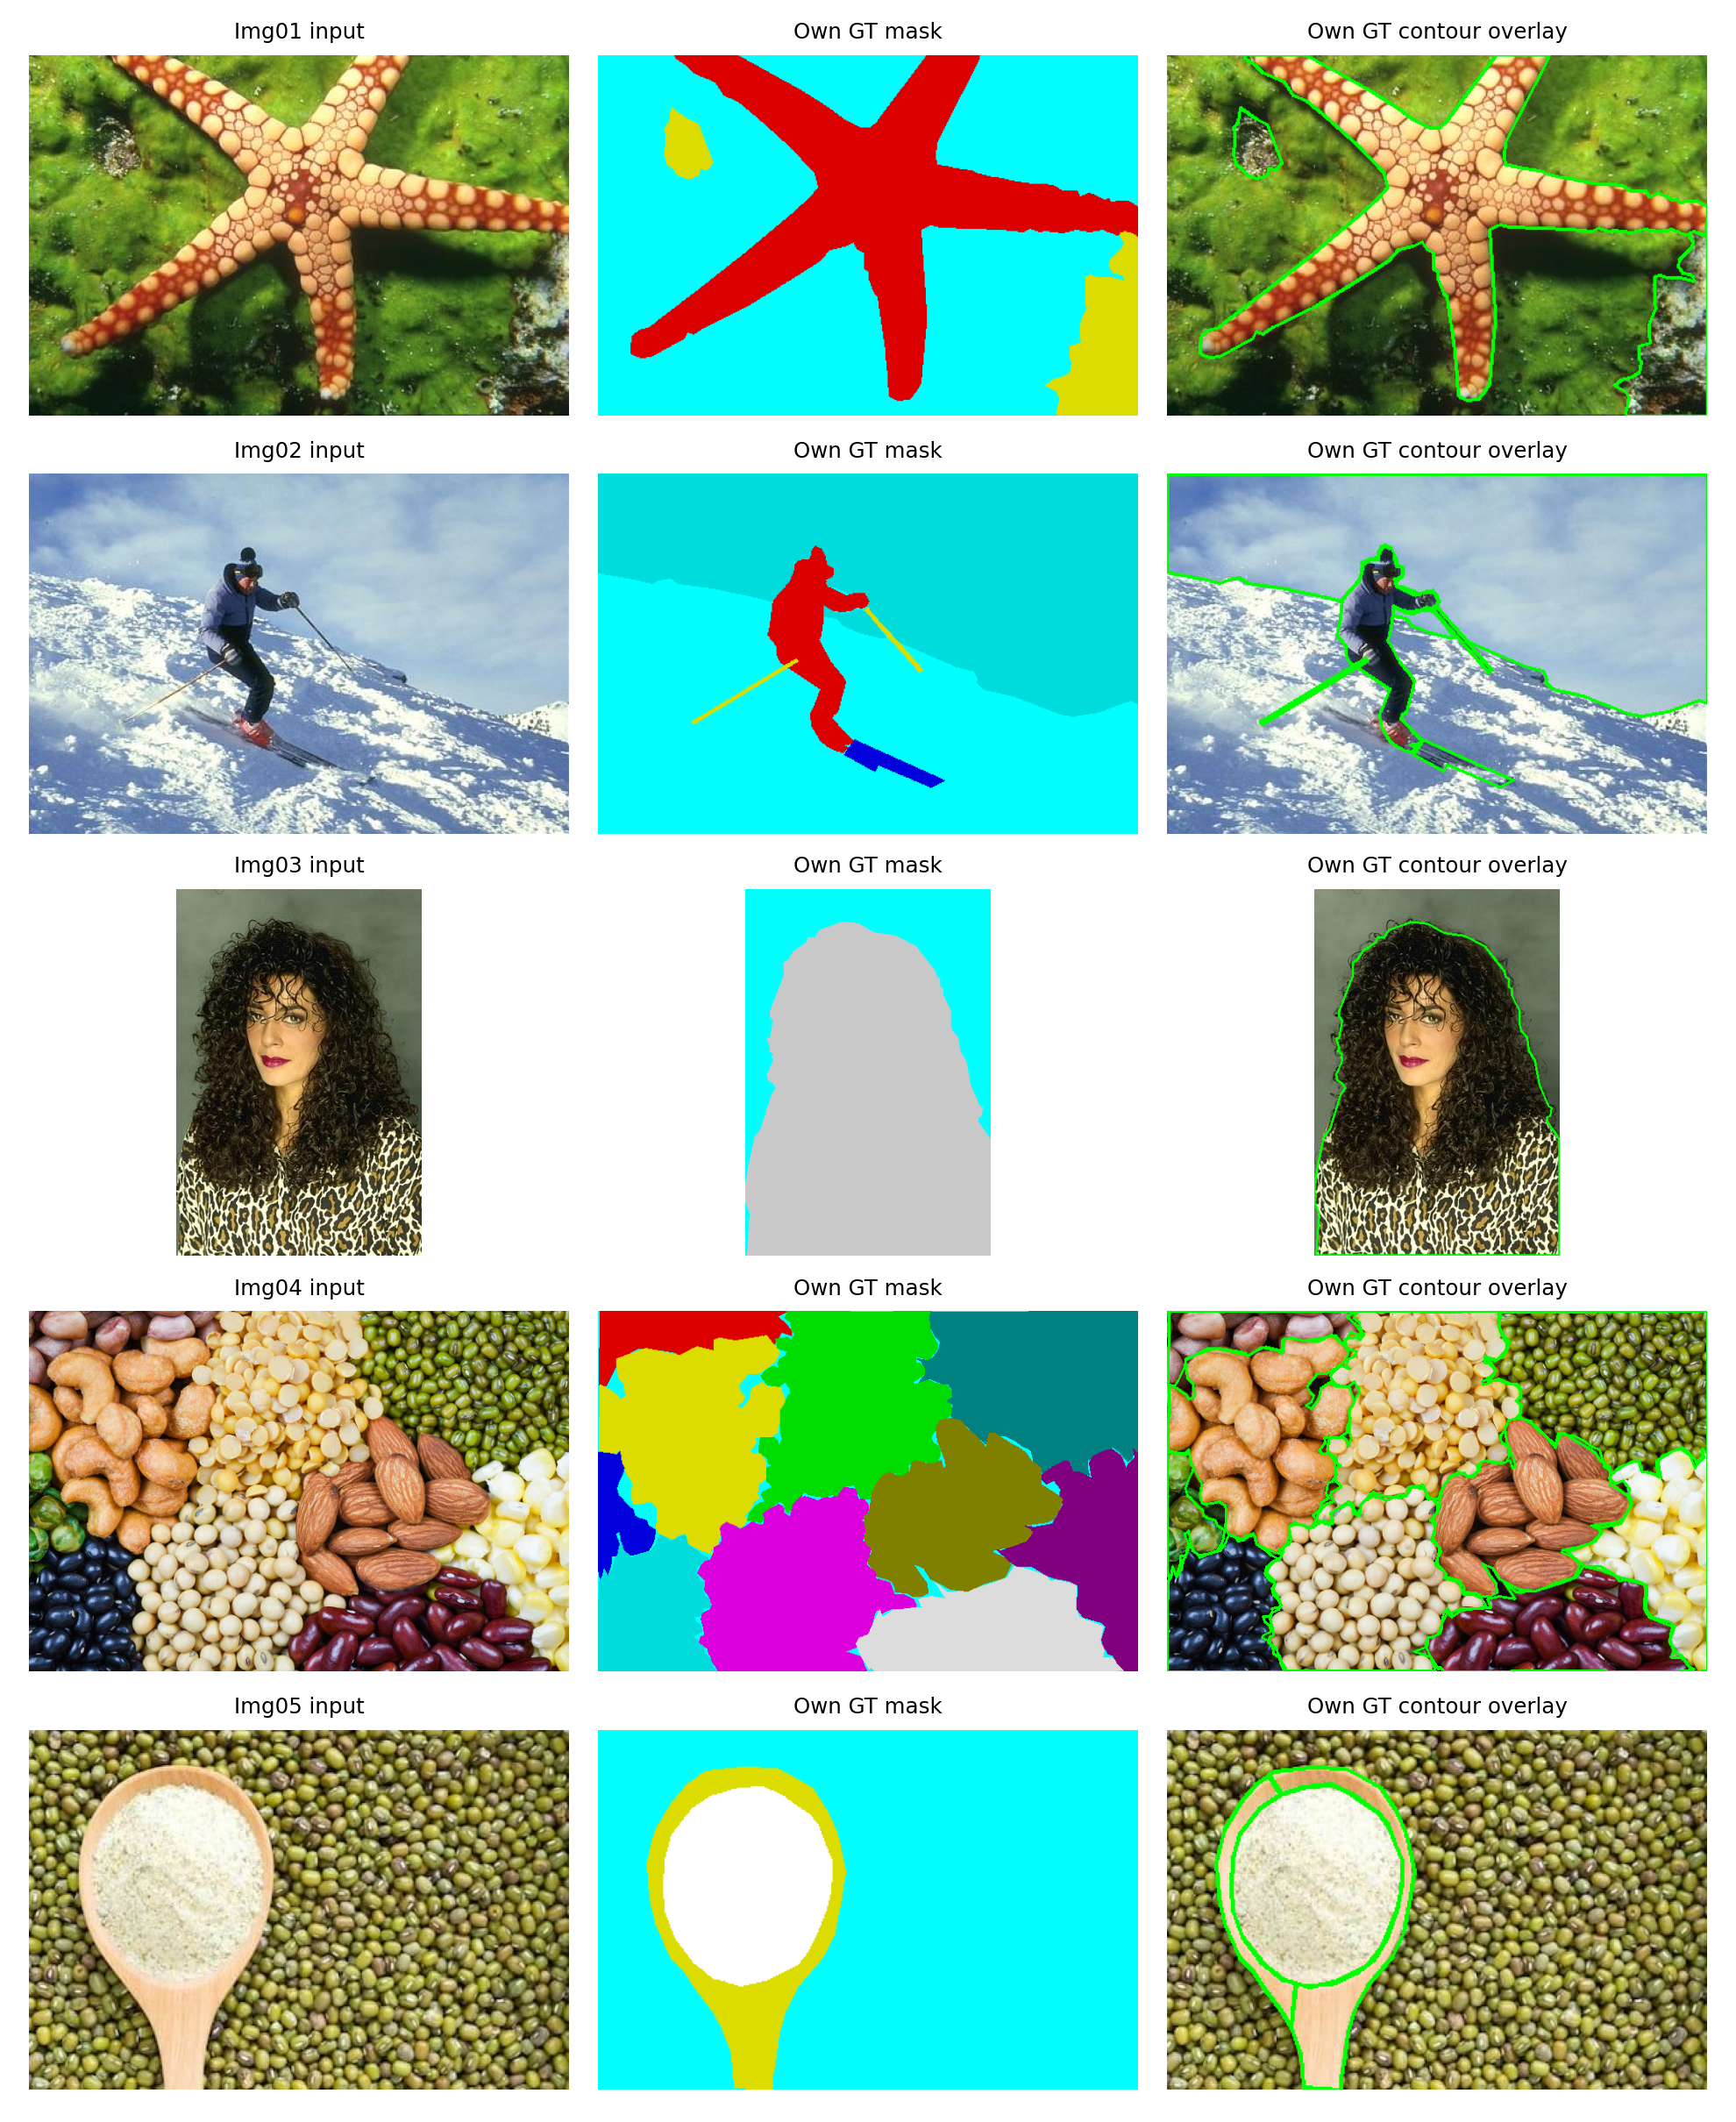
\includegraphics[width=0.88\textwidth,height=0.42\textheight,keepaspectratio]{figures/grids/own_gt_gallery_part1.png}
\caption{Self-created ground-truth examples for Images 01--05. Each row shows the input image, the filled GT mask, and the contour overlay.}
\label{fig:own-gt-gallery-a}
\end{figure}
\begin{figure}[H]
\centering
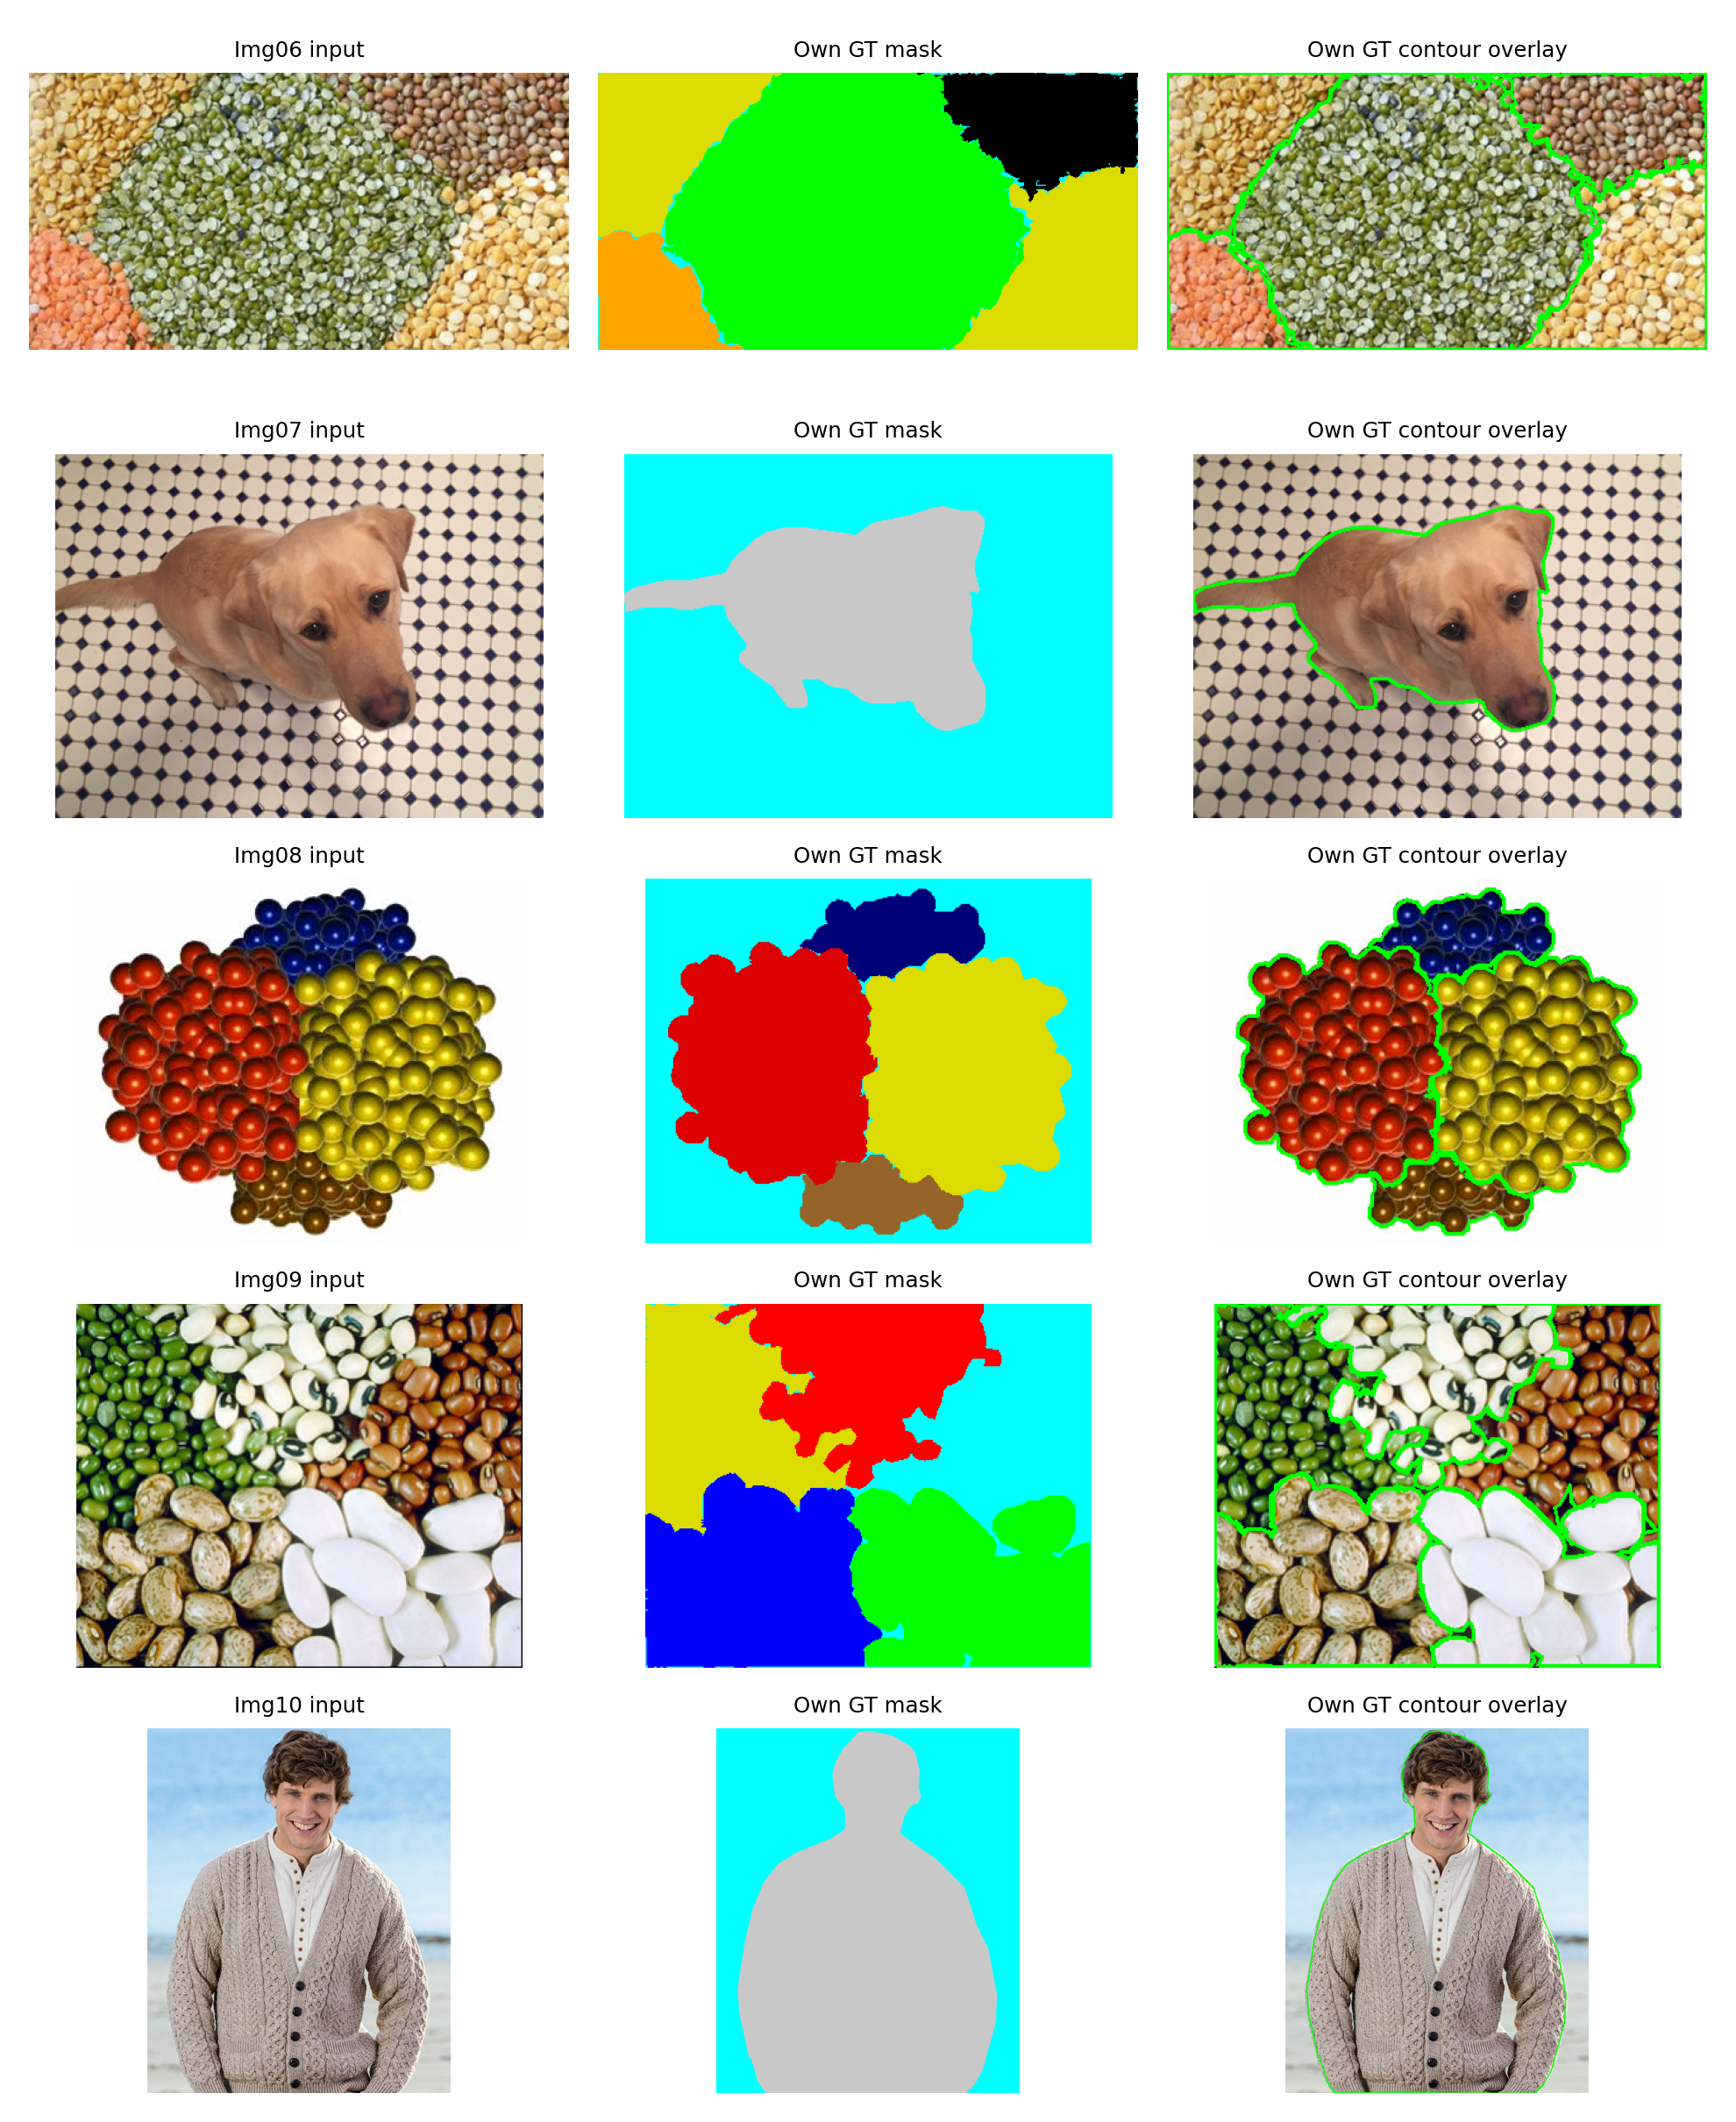
\includegraphics[width=0.88\textwidth,height=0.42\textheight,keepaspectratio]{figures/grids/own_gt_gallery_part2.png}
\caption{Self-created ground-truth examples for Images 06--10. The complete GT folders are included in \texttt{outputs/GT Ehsanul Karim/} and editable JSON files are included in \texttt{annotations/self/}.}
\label{fig:own-gt-gallery-b}
\end{figure}

\subsection{Why masks, contours, and overlays are all stored}
The mask image is used for quantitative pixel-level evaluation. The contour image is used to visually inspect boundary quality and to blend self and peer annotations. The overlay image makes the annotation quality easy to check against the input image. Keeping all three forms prevents ambiguity: masks support metrics, contours support boundary inspection, and overlays support qualitative reporting.
